\documentclass[a4paper,11pt,twoside,titlepage,openright]{book}

\usepackage[english]{babel}
\usepackage{color}
\usepackage{graphicx}
\usepackage{amsmath}
\numberwithin{equation}{section}
\usepackage[margin=3cm]{geometry}
\usepackage{hyperref}
\usepackage{epsfig,amsfonts}
\usepackage{xcolor,import}


\pagestyle{plain}

\newcommand{\ud}[1]{\underline{#1}}
\newcommand{\e}[1]{\underline{e}_{#1}}
\newcommand{\lt}{\left}
\newcommand{\rt}{\right}
\DeclareMathOperator{\L2}{L_{1/2}}
\DeclareMathOperator{\n}{\underline{n}}
\DeclareMathOperator{\ei}{\underline{e}_1}
\DeclareMathOperator{\et}{\underline{e}_2}
\DeclareMathOperator{\ex}{\underline{e}_x}
\DeclareMathOperator{\ey}{\underline{e}_y}
\DeclareMathOperator{\ez}{\underline{e}_z}
\DeclareMathOperator{\nin}{\underline{n}_{in}}
\DeclareMathOperator{\nout}{\underline{n}_{out}}
\DeclareMathOperator{\np}{\underline{n}_{P}}
\DeclareMathOperator{\bragg}{\theta_{bragg}}
\DeclareMathOperator{\DD}{\cos(\theta)^2 - \sin(\psi)^2}
\newcommand{\wdg}{\wedge}
\newcommand{\hypot}[1]{\textbf{\textcolor{green}{#1}}}


\begin{document}

\title{ToFu tools\\Magnetic fields}
\author{Didier VEZINET}
\date{05.11.2020}
\maketitle

\tableofcontents


\chapter{3D field from straight current segments}

\section{Single segment}

Let's consider current segment with current $I$, centered on $A$, with unit
vector $\ud{u}$ and half-length $\L2$. Considering a point $P$ in this segment,
identified by its length to $A$:
$$
\ud{OP} = \ud{OA} + l\ud{u},
\text{ with } l \in \left[-\L2; \L2\right]
$$

Any point $M$ in space can be located by its position with respect to $\ud{A}$
$$
\left\{
\begin{array}{ll}
    \ud{OM} = \ud{OA} + l_M\ud{u} + r_M\ud{v}\\
    \ud{v} = \ud{AM} - (\ud{AM} \cdot \ud{u}) \ud{u}
\end{array}
\right.
$$

\begin{figure}[hbtp]
    \centering
    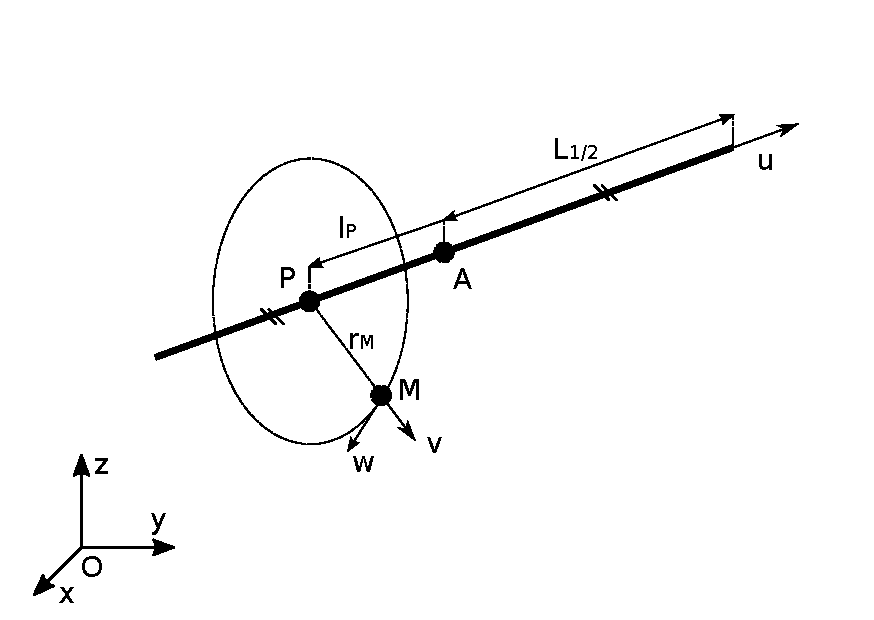
\includegraphics[scale=0.80]{Fig01_SingleSegment.pdf} 
    \caption{\small MAgnetic field at any point $M$ from a straight current
    segment}
   \label{Fig:Single}  
\end{figure}

The Biot-Savart law stipulates that an elementary length of current creates
an elementary magnetic field at $M$:
$$
\left\{
\begin{array}{ll}
\ud{dI} = Idl\ud{u}\\
\ud{PM} = (l_M-l)\ud{u} + r_M\ud{v}\\
\ud{B_A} = \frac{\mu_0}{4\pi}
	\int_{-\L2}^{\L2} \frac{\ud{dI} \wedge \ud{PM}}{\| \ud{PM}\|^3}
\end{array}
\right.
$$

Introducing $\ud{w} = \ud{u}\wedge\ud{v}$:
$$
\ud{dI}\wedge\ud{PM} = Idlr_M\ud{w}
$$

and:
$$
\|\ud{PM}\| = \sqrt{(l-l_M)^2 + r_M^2}
$$

Hence:
$$
\ud{B_A} = \frac{\mu_0}{4\pi}Ir_M\ud{w}
	\int_{-\L2}^{\L2} \frac{dl}{\left((l-l_M)^2 + r_M^2\right)^{3/2}}\\
$$

Introducing $x = l-l_M \Rightarrow dx = dl$:
$$
\begin{array}{ll}
\ud{B_A} & = \frac{\mu_0}{4\pi}Ir_M\ud{w}
	\int_{-\L2-l_M}^{\L2-l_M} \frac{dx}{\left(x^2 + r_M^2\right)^{3/2}}
\end{array}
$$

Noticing that:
$$
\begin{array}{ll}
\frac{\partial}{\partial x}\left(\frac{x}{\sqrt{x^2+a}}\right)
& = \frac{\sqrt{x^2+a} - x\frac{1}{2}\frac{2x}{\sqrt{x^2+a}}}{x^2+a}\\
& = \frac{(x^2+a) - x^2}{(x^2+a)^{3/2}}\\
& = \frac{a}{(x^2+a)^{3/2}}
\end{array}
$$

Hence:
$$
\begin{array}{ll}
\ud{B_A} & = \frac{\mu_0}{4\pi}Ir_M\ud{w}
	\left[\frac{1}{r_M^2}\frac{x}{\sqrt{x^2+r_M^2}}\right]_{-\L2-l_M}^{\L2-l_M}\\
	& =  \frac{\mu_0}{4\pi}\frac{I}{r_M}\ud{w}
	\left(\frac{\L2-l_M}{\sqrt{(\L2-l_M)^2+r_M^2}}
	+ \frac{\L2+l_M}{\sqrt{(\L2+l_M)^2+r_M^2}}\right)\\
\end{array}
$$

For numerical evaluation, keep in mind that:
$$
\left\{
\begin{array}{ll}
l_M = \ud{u}\cdot\ud{AM}\\
r_M = \|\ud{u}\wedge\ud{AM}\|\\
\ud{w} = \frac{\ud{u}\wedge\ud{AM}}{r_M}
\end{array}
\right.
$$


\section{2 mirrored segments}

Let's consider 2 current segments $(A, \ud{u})$ and $(A', \ud{u'})$ one being
the symmetric of the other via a symmetry plane $(M, \ud{n})$.\\
Each current segment has its own current $I$ (resp. $I'$).

\begin{figure}[hbtp]
    \centering
    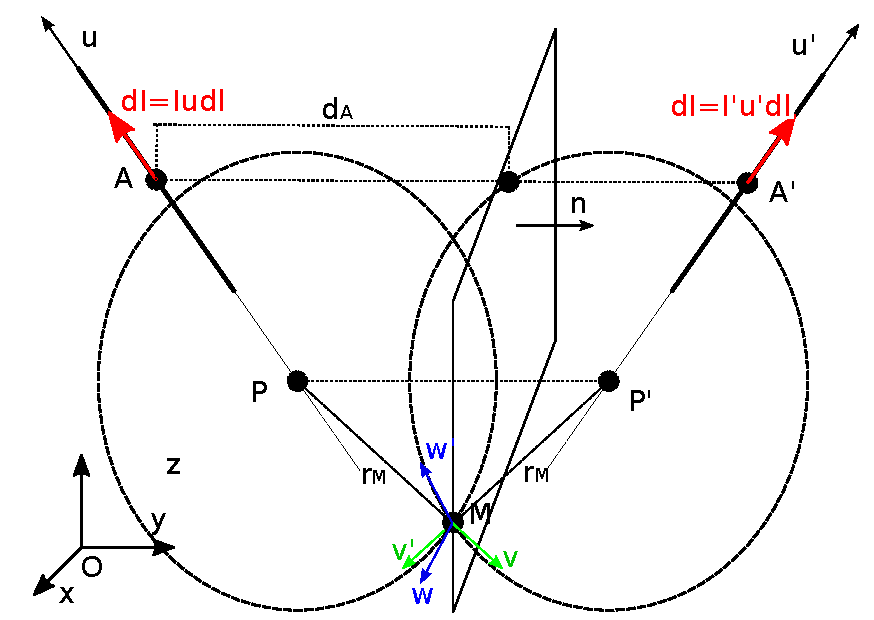
\includegraphics[scale=0.50]{Fig02_MirroredSegments.pdf} 
    \caption{\small Magnetic field at any point $M$ from 2 mirrored straight
    current segments}
   \label{Fig:Mirrored}  
\end{figure}

By construction:
$$
\left\{
\begin{array}{lll}
    l'_P & = l_M\\
    r'_M & = r_M\\
    L'_{1/2} & = L_{1/2}\\
    d_A & = \ud{AM} \cdot \ud{n}\\
    \ud{AA'} & = 2d_A\ud{n}\\
    \ud{u}' & = \ud{u} - 2(\ud{u} \cdot \ud{n})\ud{n}\\
    \ud{AM} & = l_M\ud{u} + r_M\ud{v}\\
    \ud{A'M} & = l_M\ud{u'} + r_M\ud{v'}\\
\end{array}
\right.
$$


The total magnetic field created in $M$ is:
$$
\begin{array}{lll}
    \ud{B}
    & = \ud{B_A}(I) + \ud{B_{A'}}(I')\\
	& =  \frac{\mu_0}{4\pi}\frac{I}{r_M}\ud{w}
	\left(\frac{\L2-l_M}{\sqrt{(\L2-l_M)^2+r_M^2}}
	+ \frac{\L2+l_M}{\sqrt{(\L2+l_M)^2+r_M^2}}\right)
	+ \frac{\mu_0}{4\pi}\frac{I'}{r_M}\ud{w'}
	\left(\frac{\L2-l_M}{\sqrt{(\L2-l_M)^2+r_M^2}}
	+ \frac{\L2+l_M}{\sqrt{(\L2+l_M)^2+r_M^2}}\right)\\
	& =  \frac{\mu_0}{4\pi}\frac{1}{r_M}
	\left(\frac{\L2-l_M}{\sqrt{(\L2-l_M)^2+r_M^2}}
	+ \frac{\L2+l_M}{\sqrt{(\L2+l_M)^2+r_M^2}}\right)
    \left(I\ud{w} + I'\ud{w'}\right)
\end{array}
$$

Now, considering that:
$$
\begin{array}{llll}
    & r_M\ud{v'}
    & = \ud{A'M}-l_M\ud{u'}\\
    && = \ud{A'A} + \ud{AM} - l_M(\ud{u} - 2(\ud{u}\cdot\ud{n})\ud{n})\\
    && = -2d_A\ud{n} + \ud{AM} - l_M\ud{u} + 2l_M(\ud{u}\cdot\ud{n})\ud{n}\\
    && = -2d_A\ud{n} + r_M\ud{v} + 2l_M(\ud{u}\cdot\ud{n})\ud{n}\\
    \Leftrightarrow
    & \ud{v'}
    & = \ud{v} + \frac{2}{r_M}\left(l_M(\ud{u}\cdot\ud{n}) - d_A\right)\ud{n}
\end{array}
$$

Hence:
$$
\begin{array}{lll}
    \ud{w'}
    & = \ud{u'} \wedge \ud{v'}\\
    & = (\ud{u} - 2(\ud{u}\cdot\ud{n})\ud{n})
    \wedge
    \left(\ud{v} + \frac{2}{r_M}\left(l_M(\ud{u}\cdot\ud{n}) - d_A\right)\ud{n}\right)\\
    & = \ud{u}\wedge\ud{v}
    + \frac{2}{r_M}\left(l_M(\ud{u}\cdot\ud{n}) - d_A\right)\ud{u}\wedge\ud{n}
    - 2(\ud{u}\cdot\ud{n})\ud{n}\wedge\ud{v}\\
    & = \ud{w}
    + 2\left[\frac{(\ud{u}\cdot\ud{n})l_M - d_A}{r_M}\ud{u}
    + (\ud{u}\cdot\ud{n})\ud{v}\right] \wedge \ud{n}\\
    & = \ud{w}
    + 2\left[\frac{(\ud{u}\cdot\ud{n})(l_M\ud{u}+r_M\ud{v}) - d_A\ud{u}}{r_M}
    \right] \wedge \ud{n}\\
    & = \ud{w}
    + 2\left[\frac{(\ud{u}\cdot\ud{n})\ud{AM} - d_A\ud{u}}{r_M}\right]
    \wedge \ud{n}
\end{array}
$$

Then, assuming $I'=-I$ we have:
$$
\begin{array}{lll}
    \ud{B}
	& =  \frac{\mu_0}{4\pi}\frac{I}{r_M}
	\left(\frac{\L2-l_M}{\sqrt{(\L2-l_M)^2+r_M^2}}
	+ \frac{\L2+l_M}{\sqrt{(\L2+l_M)^2+r_M^2}}\right)
    \left(\ud{w} - \ud{w'}\right)\\
	& = -\frac{\mu_0}{4\pi}\frac{I}{r_M}
	\left(\frac{\L2-l_M}{\sqrt{(\L2-l_M)^2+r_M^2}}
	+ \frac{\L2+l_M}{\sqrt{(\L2+l_M)^2+r_M^2}}\right)
    \left(2\left[\frac{(\ud{u}\cdot\ud{n})\ud{AM} - d_A\ud{u}}{r_M}\right]
    \wedge \ud{n}\right)\\
	& = \frac{\mu_0}{2\pi}\frac{I}{r_M}
	\left(\frac{\L2-l_M}{\sqrt{(\L2-l_M)^2+r_M^2}}
	+ \frac{\L2+l_M}{\sqrt{(\L2+l_M)^2+r_M^2}}\right)
    \left(
    \ud{n} \wedge \left[\frac{(\ud{u}\cdot\ud{n})\ud{AM} - d_A\ud{u}}{r_M}\right]
    \right)\\
\end{array}
$$

For numerical evaluation, keep in mind that:
$$
\left\{
\begin{array}{ll}
l_M = \ud{u}\cdot\ud{AM}\\
r_M = \|\ud{u}\wedge\ud{AM}\|\\
    d_A = \ud{AM}\cdot\ud{n}
\end{array}
\right.
$$


\section{4 mirrored segments}

Let's consider the 2 previous mirrored current segments and add a pair
mirroring them via another plane $(C, \ud{m})$, perpendicular to the first
plane $(C, \ud{n})=(M, \ud{n})$. All segments are lying in the same plane $(C, \ud{a})$\\
The same current is running through each segment and they all have the same
half-length $L_{1/2}$.\\

The same derivation as previously can be done for pair $AA'$ and pair $BB'$.

\begin{figure}[hbtp]
    \centering
    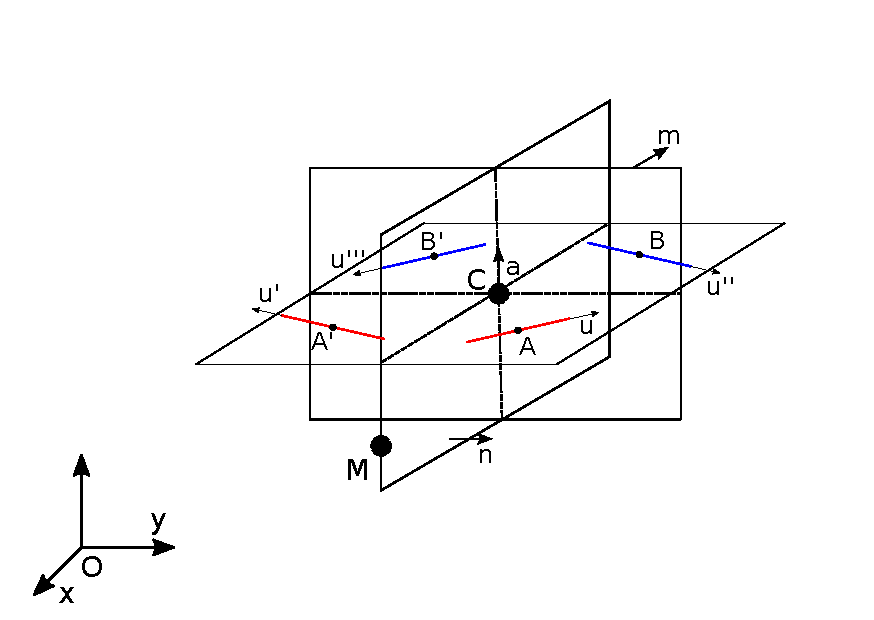
\includegraphics[scale=0.80]{Fig03_SegmentedCircle.pdf} 
    \caption{\small Magnetic field at any point $M$ from 2 mirrored straight
    current segments}
   \label{Fig:Mirrored}  
\end{figure}

The total magnetic field created in $M$ is:
$$
\begin{array}{lll}
    \ud{B}
    & = \ud{B_{AA'}}(I) + \ud{B_{BB'}}(I)\\
	& = \frac{\mu_0}{2\pi}\frac{I}{r_M}
	\left(\frac{\L2-l_M}{\sqrt{(\L2-l_M)^2+r_M^2}}
	+ \frac{\L2+l_M}{\sqrt{(\L2+l_M)^2+r_M^2}}\right)
    \left(
    \ud{n} \wedge \left[\frac{(\ud{u}_A\cdot\ud{n})\ud{AM} - d_A\ud{u}_A}{r_M}\right]
    \right)\\
	& + \frac{\mu_0}{2\pi}\frac{I}{r_M''}
	\left(\frac{\L2-l_M''}{\sqrt{(\L2-l_M'')^2+r_M''^2}}
	+ \frac{\L2+l_M''}{\sqrt{(\L2+l_M'')^2+r_M''^2}}\right)
    \left(
    \ud{n} \wedge \left[\frac{(\ud{u}_B\cdot\ud{n})\ud{BM} - d_B\ud{u}_B}{r_M''}\right]
    \right)\\
\end{array}
$$

By construction, we have:
.... cannot get $(r''_M, l''_M)$ from $(r_M, l_M)$.



\chapter{Circular coil}
\label{chap:CircularCoil}

The magnetic field produced at any point in 3D space by a planar circular coil
cannot be derived analytically.


\section{Circle discretization}

Let's consider a circular coil of radius $R$ centered on axis $(A, \ud{n})$.

For a given point $M$ in space, let's make the plane $(O, M, \ud{e}_z)$ a
symmetry plane and divide the circle into a $N$-sided polygon.

\subsection{N-sided polygon}
\label{subsect:constraint}

The polygon is N-sided, with N an even number.
The polygon shall have either:
\begin{itemize}
	\item the same perimeter as the circle: $L=2\pi R$
	\item the same area as the circle: $S=\pi R^2$
    \item the same magnetic field on the center as the circle:
        $B=\frac{\mu_0I}{2R}$
\end{itemize}

For a N-sided regular polygon of height $h$:
$$
\left\{
    \begin{array}{ll}
	    L_i = 2h\tan\left(\frac{\pi}{N}\right) & \text{ is the length a single side}\\
		S_i = \frac{hL_i}{2} = h^2\tan\left(\frac{\pi}{N}\right) & \text{ is the area a single side}
	\end{array}
\right.
$$

Remembering that, at the center, $l_m=0$ and $r_m=h$ for all, by construction,
and that $\L2=\frac{L_i}{2}=h\tan\left(\frac{\pi}{N}\right)$, we derive:
$$
\begin{array}{ll}
    B & = N \frac{\mu_0}{4\pi}\frac{I}{h}
    \left(\frac{\L2}{\sqrt{(\L2)^2+h^2}}
    + \frac{\L2}{\sqrt{(\L2)^2+h^2}}\right)\\
    & = N \frac{\mu_0}{2\pi}\frac{I}{h}
    \frac{\L2}{\sqrt{(\L2)^2+h^2}}\\
    & = N \frac{\mu_0}{2\pi}\frac{I}{h}
    \frac{h\tan\left(\frac{\pi}{N}\right)}{\sqrt{h^2\tan^2\left(\frac{\pi}{N}\right)+h^2}}\\
    & = N \frac{\mu_0}{2\pi}\frac{I}{h}
    \frac{\tan\left(\frac{\pi}{N}\right)}{\sqrt{\tan^2\left(\frac{\pi}{N}\right)+1}}\\
    & = \frac{\mu_0I}{2}\frac{1}{h}\frac{N}{\pi}
    \frac{\tan\left(\frac{\pi}{N}\right)}{\sqrt{\tan^2\left(\frac{\pi}{N}\right)+1}}\\
\end{array}
$$

Hence,
\begin{itemize}
	\item same perimeter
        $\Rightarrow h = R \frac{\frac{\pi}{N}}{\tan\left(\frac{\pi}{N}\right)}$
	\item same area
        $\Rightarrow h = R \sqrt{\frac{\frac{\pi}{N}}{\tan\left(\frac{\pi}{N}\right)}}$
    \item same field
        $\Rightarrow h =
        R\frac{\tan\left(\frac{\pi}{N}\right)}{\frac{\pi}{N}}\frac{1}{\sqrt{\tan^2\left(\frac{\pi}{N}\right)+1}}$
\end{itemize}


\subsection{Symetries}

Let's consider, for a point $M$, the 2 symetry planes passing through the
center of the circle, containing its axis, and one passing through $M$, the
other one perpendicular to that one.

This way we can define a 4-symetry for the discretization of the circle,
indexed by $n$.


\subsection{Deriving B from discretized 3D cirle}

Let's consider a spire as a circle in 3D with center $C$, axis $(C, \ud{e}_3)$
and radius $R$.
Let's consider a point $M$ in 3D with coordinates $(x_M, y_M, z_M)$.

Local coordinate system $(\ud{e}_1, \ud{e}_2)$ can be defined from:
$$
\left\{
    \begin{array}{ll}
        \ud{CM} = r\ud{e}_1 + z\ud{e}_3\\
        \ud{e}_2 = \ud{e}_3 \wedge \ud{e}_1
	\end{array}
\right.
$$

Let's discretize the circle into a 4n-sided polygon with 2 symetry planes,
including $(M, C, {e}_3)$.

Depending on the constraint, the height $h$ of each polygon can be derived (cf.
~\ref{subsect:constraint}). Similarly, the length of the basis of each polygon
can also be derived as $L=2h\tan(\frac{\pi}{4n})$.

Knowing $h$ and $L$ one can write, for $i \in [1; 2n]$ (we only consider one
half of the circle due to the symetry):
$$
\left\{
    \begin{array}{ll}
        \theta_i = (i-\frac{1}{2})\frac{\pi}{4n}\\
        \ud{CA_i} = h\cos(\theta_i)\ud{e}_1 + h\sin(\theta_i)\ud{e}_2\\
        \ud{u}_i = -\sin(\theta_i)\ud{e}_1 + \cos(\theta_i)\ud{e}_2\\
	\end{array}
\right.
$$

For each side $i$, we can write:
$$
\begin{array}{ll}
    \ud{A_iM}
    & = \ud{CM} - \ud{CA_i}\\
    & = r\ud{e}_1 + z\ud{e}_3
    - h\cos(\theta_i)\ud{e}_1 - h\sin(\theta_i)\ud{e}_2\\
    & = (r-h\cos(\theta_i))\ud{e}_1 - h\sin(\theta_i)\ud{e}_2 + z\ud{e}_3
\end{array}
$$

Hence:
$$
\begin{array}{lll}
    \ud{u}_i \wedge \ud{A_iM}
    & = & (-\sin(\theta_i))(- h\sin(\theta_i))\ud{e}_3
    + (-\sin(\theta_i))(z)(-\ud{e}_2)\\
    && + (\cos(\theta_i))((r-h\cos(\theta_i)))(-\ud{e}_3)
    + (\cos(\theta_i))(z)(\ud{e}_1)\\
    & = & z\cos(\theta_i)\ud{e}_1
    + z\sin(\theta_i)\ud{e}_2
    + (h\sin^2(\theta_i) + h\cos^2(\theta_i) - r\cos(\theta_i))\ud{e}_3\\
    & = & z\cos(\theta_i)\ud{e}_1
    + z\sin(\theta_i)\ud{e}_2
    + (h - r\cos(\theta_i))\ud{e}_3\\
\end{array}
$$

and:
$$
\begin{array}{lll}
    \ud{u}_i \cdot \ud{A_iM}
    & = & (r-h\cos(\theta_i))(-\sin(\theta_i))
    + (\cos(\theta_i))(-h\sin(\theta_i))\\
    & = & -r\sin(\theta_i)
\end{array}
$$

And since here $\ud{n} = \ud{e}_2$:
$$
\begin{array}{lll}
    \ud{A_iM} \cdot \ud{n}
    & = & - h\sin(\theta_i)\\
\end{array}
$$

Hence:
$$
\left\{
    \begin{array}{lll}
        r_{Mi} & = \sqrt{z^2 + (h - r\cos(\theta_i))^2}\\
        l_{Mi} & = -r\sin(\theta_i)\\
        d_{Ai} & = - h\sin(\theta_i)
    \end{array}
\right.
$$




\appendix
\chapter{Appendices}

\section{Section}
\subsection{Subsection}

\end{document}
